\documentclass{standalone}
\usepackage{tikz}

\usetikzlibrary{calc,math}


\begin{document}

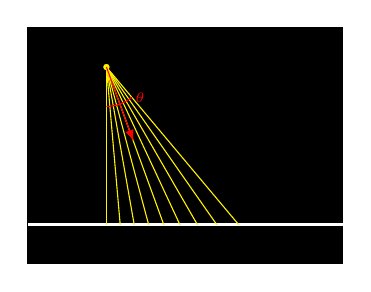
\begin{tikzpicture}
  \tikzmath{
    real \startangle;
    \startangle=-70;
  }
  \coordinate (light) at (-1,2);

  \path[use as bounding box] (-2,-0.5) rectangle (2,2.5);
  \draw[fill=black] (-2,-0.5) rectangle (2,2.5);
  \draw[white!10,thick] (-2,0) -- (2,0);
  \draw[fill=yellow] (light) circle [radius=0.05cm];

  \begin{scope}
    \path[clip] (-2,0) rectangle (2,4);
    \foreach \x in {-20,-15,...,20} {
      \draw[yellow] (light) -- ++(\startangle+\x:5);
    }
  \end{scope}

  \draw[-latex,red] (light) -- ++(\startangle:1);
  \draw[red] ($ (light) + (\startangle-20:0.5) $) arc [start angle=-90,delta angle=40,radius=0.5] node[right,font=\tiny,inner sep=1pt] {$\theta$};
\end{tikzpicture}

\end{document}